% Created 2019-12-05 Thu 22:44
% Intended LaTeX compiler: pdflatex
\documentclass[11pt]{article}
\usepackage[utf8]{inputenc}
\usepackage[T1]{fontenc}
\usepackage{graphicx}
\usepackage{grffile}
\usepackage{longtable}
\usepackage{wrapfig}
\usepackage{rotating}
\usepackage[normalem]{ulem}
\usepackage{amsmath}
\usepackage{textcomp}
\usepackage{amssymb}
\usepackage{capt-of}
\usepackage{hyperref}
\author{Heitor Lourenço Werneck \\{\href{mailto:heitorwerneck@hotmail.com}{heitorwerneck@hotmail.com}}}
\usepackage[portuguese]{babel}
\usepackage{mathtools}
\usepackage[binary-units=true]{siunitx}
\usepackage[top=0.5cm,bottom=1.5cm,left=2cm,right=2cm]{geometry}
\usepackage{mdframed}
\usepackage{listings}
\usepackage[noend]{algpseudocode}
\usepackage{algorithm}
\usepackage{tikz}
\usepackage{xcolor}
\usepackage{colortbl}
\usepackage{graphicx,wrapfig,lipsum}
\RequirePackage{fancyvrb}
\DefineVerbatimEnvironment{verbatim}{Verbatim}{fontsize=\small}
\usepackage[font=small,labelfont=bf]{caption} % Required for specifying captions to tables and figures
\usepackage[subrefformat=parens]{subcaption}
\date{\today}
\title{Cálculo numérico\\\medskip
\large Trabalho Prático 1}
\hypersetup{
 pdfauthor={Heitor Lourenço Werneck},
 pdftitle={Cálculo numérico},
 pdfkeywords={},
 pdfsubject={},
 pdfcreator={Emacs 26.3 (Org mode 9.1.9)}, 
 pdflang={Portuguese}}
\begin{document}

\maketitle
\tableofcontents

\usetikzlibrary{arrows, fit, matrix, positioning, shapes, backgrounds,intersections}
\usetikzlibrary{decorations.pathreplacing}
\usetikzlibrary{automata, positioning, arrows}
\usetikzlibrary{calc}

\definecolor{bg}{rgb}{0.95,0.95,0.95}
\BeforeBeginEnvironment{minted}{\begin{mdframed}[backgroundcolor=bg]}
\AfterEndEnvironment{minted}{\end{mdframed}}
\numberwithin{equation}{section}
\algnewcommand{\IfThenElse}[3]{% \IfThenElse{<if>}{<then>}{<else>}
  \State \algorithmicif\ #1\ \algorithmicthen\ #2\ \algorithmicelse\ #3}

% Define block styles
\tikzstyle{decision} = [diamond, draw, fill=blue!20, 
    text width=4.5em, text badly centered, node distance=3cm, inner sep=0pt]
\tikzstyle{block} = [rectangle, draw, fill=blue!20, 
    text width=5em, text centered, rounded corners, minimum height=4em]
\tikzstyle{line} = [draw, -latex']
\tikzstyle{cloud} = [ellipse, draw, fill=red!20, 
    text width=5em, text centered, rounded corners, minimum height=2em]
%\tikzstyle{cloud} = [draw, ellipse,fill=red!20, node distance=3.5cm,
%    minimum height=2em]


\lstset{
  basicstyle=\ttfamily,
  columns=fullflexible,
  frame=single,
  breaklines=true,
  postbreak=\mbox{\textcolor{red}{$\hookrightarrow$}\space},
}
\DeclarePairedDelimiter\ceil{\lceil}{\rceil}
\DeclarePairedDelimiter\floor{\lfloor}{\rfloor}

\section{Introdução}
\label{sec:org5b61ef1}

Regressão linear múltipla é um método estatístico que permite a criação de um modelo linear com diversas variáveis que descreve ou se a aproxima do comportamento dos dados de entrada.

A aplicação de regressão linear múltipla é das mais diversas como por exemplo: previsão de preço de casas, previsão de temperatura máxima em um dia e previsão de valor de itens com base em algumas de suas características. 

Esse trabalho tem como objetivo aplicar o método de regressão linear com múltiplas variáveis em uma base, que no caso é uma base de 50 \emph{startups} e o objetivo será predizer o ganho das \emph{startups}.

\section{Base de dados}
\label{sec:org9999818}

A base de dados contem as informações mostradas na tabela \ref{tab:cols}, um problema para a regressão seria o tipo texto porém essa variável pode ser transformada para variáveis \emph{dummies} tal que se o valor na tabela original for ``New York`` somente uma variável ``State\_New York`` terá valor 1 e as outras 0, essa lógica é mostrada na tabela \ref{tab:dummies}.

\begin{table}[htbp]
\centering
\begin{tabular}{ll}
Coluna & Tipo\\
\hline
R\&D Spend & Ponto flutuante\\
Administration & Ponto flutuante\\
Marketing Spend & Ponto flutuante\\
State & Texto\\
Profit & Ponto flutuante\\
\hline
\end{tabular}
\caption{\label{tab:cols}
Dados na base.}

\end{table}


\begin{table}[htbp]
\centering
\begin{tabular}{cccc}
State & State\_New York & State\_California & State\_Florida\\
\hline
New York & 1 & 0 & 0\\
California & 0 & 1 & 0\\
Florida & 0 & 0 & 1\\
\hline
\end{tabular}
\caption{\label{tab:dummies}
Variáveis \emph{dummies}, mapeamento de valores.}

\end{table}


\subsection{Análise}
\label{sec:org6f0371b}

O número de amostras dessa base é 50 como dito na introdução, para o contexto de aprendizado de maquina não é muito porém será o suficiente para esse caso.

Uma visão geral da base de dados é dada na figura \ref{fig:data_set}, como pode ser visto pela média a cidade com menos \emph{startups} é a florida.

A magnitude dos valores são grandes como pode ser visto nas outras colunas.

O desvio padrão do gasto em ``Administration`` é o menor comparado aos outros valores.

Em ``R\&D Spend`` e ``Marketing Spend`` existe \emph{startup} com 0, que pode ser considerado uma empresa que não tem motivo de gastar nesses campos e talvez seja um \emph{outlier} da base de dados.

Já em ``Profit`` e ``Administration`` todos tiveram valores maiores que 0.

A maior média de gasto de todas empresas é em ``Marketing`` mesmo que algumas empresas não gastem com essa parte o valor de todas outras empresas que gastam compensa.

Após ser feito uma regressão será possível inferir, não com completa exatidão, qual o gasto que mais gera lucro.

\begin{figure}[htbp]
\centering
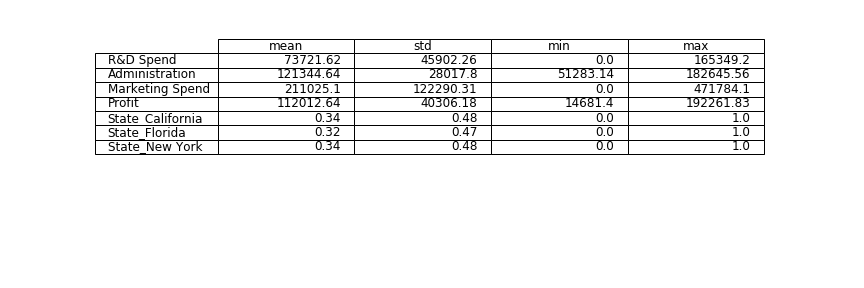
\includegraphics[width=.9\linewidth]{./data_set.png}
\caption{\label{fig:data_set}
Medidas da base de dados.}
\end{figure}


\section{Modelagem e solução}
\label{sec:orgf2ec1eb}

Para ser feito a regressão linear com múltiplas variáveis será utilizado o modelo \(G^T\cdot G\cdot \alpha = G^T\cdot y\) que dará o modelo com menor distância dos pontos dados (método dos mínimos quadrados) tal que \(y\) é uma matriz coluna da variável a ser predita, \(G\) é a matriz da base de dados, porém sem a coluna da característica a ser predita, e \(\alpha\) é os parâmetros a serem descobertos para criação da função preditora.

No caso para ser realizado essas operações é necessário definir o transposto de uma matriz e a multiplicação de matrizes.

Para ser feito a transposta da matriz é utilizado o algoritmo \ref{alg:transpose}.

\begin{algorithm}
\caption{Matriz transposta.}\label{alg:transpose}
\begin{algorithmic}[1]
\Procedure{Transposta}{$Matriz$}
\State $Matriz^T \gets NovaMatriz(Matriz.colunas,Matriz.linhas)$ \Comment{Cria matriz com ``$Matriz.colunas$`` colunas e ``$Matriz.linhas$`` linhas}
\For{$j=0$ \textbf{to} $Matriz.colunas-1$}
\For{$i=0$ \textbf{to} $Matriz.linhas-1$}
\State $Matriz^T[j,i] = Matriz[i,j]$
\EndFor
\EndFor
\State \textbf{return} $Matriz^T$
\EndProcedure
\end{algorithmic}
\end{algorithm}


O algoritmo \ref{alg:multiply} descreve o funcionamento da multiplicação de matrizes.
O ponto fundamental do algoritmo ocorre na linha \ref{alg:multiply:mainfor} que é o laço que soma a multiplicação dos elementos da linha \(i\) da matriz 1 com os elementos da coluna \(j\) da matriz 2 e atribui essa soma na linha \ref{alg:multiply:soma} a posição \(i\) e \(j\) da matriz resultante.

\begin{algorithm}
\caption{Multiplicação de matrizes.}\label{alg:multiply}
\begin{algorithmic}[1]
\Procedure{Multiplicacao}{$M1,M2$}
\State $MResultante \gets NovaMatriz(M1.linhas,M2.colunas)$ \Comment{Cria matriz com zeros}
\For{$i=0$ \textbf{to} $MResultante.linhas-1$}
\For{$j=0$ \textbf{to} $MResultante.colunas-1$}
\State $soma = 0$
\For{$k=0$ \textbf{to} $M1.colunas-1$}\label{alg:multiply:mainfor}
\State $soma \gets soma + M1[i,k] \cdot M2[k,j]$
\EndFor
\State $MResultante[i,j] \gets soma$\label{alg:multiply:soma}
\EndFor
\EndFor
\State \textbf{return} $MResultante$
\EndProcedure
\end{algorithmic}
\end{algorithm}


Após ser feito a transposta e multiplicação da matriz só falta um método para solucionar um sistema de equação linear.

O método escolhido foi o Gauss-Seidel pois o mesmo é eficiente e converge rápido.
O algoritmo \ref{alg:gaussseidel} mostra o funcionamento.


\begin{algorithm}
  \caption{Método de resolução de sistema de equação linear.}\label{alg:gaussseidel}
  \begin{algorithmic}[1]
    \Procedure{GaussSeidel}{$A,b,Erro = 0.0001$}
    \State $X_{Velho} \gets [0..b.linhas-1]$ \Comment{Começa com todos elementos iguais a zero}
    \State $DistanciaMaxima \gets \infty$
    \While {$DistanciaMaxima>Erro$}
        \State $X_{Novo} \gets [0..b.linhas-1]$
        \For{$i=0$ \textbf{to} $A.linhas-1$}
            \State $X_{Novo}[i] \gets b[i][0]$
            \For{$j=0$ \textbf{to} $A.colunas-1$}
                \If {$i\neq j$}
                    \If {$j<i$}
                        \State $X_{Novo}[i] \gets X_{Novo}[i] - A[i][j]\cdot X_{Novo}[j]$
                    \Else
                        \State $X_{Novo}[i] \gets X_{Novo}[i] - A[i][j]\cdot X_{Velho}[j]$
                    \EndIf
                \EndIf
            \EndFor
	    \State $X_{Novo}[i] \gets X_{Novo}[i]/A[i][i]$
        \EndFor
    \State $DistanciaMaxima \gets 0$
    \For{$i=0$ \textbf{to} $b.linhas-1$}\Comment{Calcula o erro pela distância}
    \State $DistanciaMaxima \gets max(DistanciaMaxima,|X_{Novo}[i] - X_{Velho}[i]|)$
    \EndFor
    \State $X_{Velho} \gets X_{Novo}$
    \EndWhile
    \State \textbf{return} $X_{Novo}$
    \EndProcedure
  \end{algorithmic}
\end{algorithm}

Com todos esses componentes e métodos basta utilizá-los para solucionar o problema. O algoritmo \ref{alg:regression} é a solução final para o problema.

\begin{algorithm}
  \caption{Regressão linear com múltiplas variáveis.}\label{alg:regression}
  \begin{algorithmic}[1]
    \Procedure{RegressaoLinear}{$G,y$}
    \State $G^T \gets Transposta(G)$
    \State $G^TG \gets Multiplicacao(G^T,G)$
    \State $G^Ty \gets Multiplicacao(G^T,y)$
    \State $Parametros \gets GaussSeidel(G^TG,G^Ty)$
    \EndProcedure
  \end{algorithmic}
\end{algorithm}


\section{Análise de resultados}
\label{sec:org7ef48bc}

Primeiro foi separado os dados em 70\% para treino e 30\% para teste.

O treino foi utilizado para treinamento do modelo com o algoritmo de regressão linear com múltiplas variáveis apresentado.

Depois do treinamento a função preditora da equação \ref{eq:predictedfunction} foi obtida.

\begin{equation}\label{eq:predictedfunction}
\begin{aligned}
Profit(R\&D Spend,Administration,...) = (0.823)*R\&D Spend+(-0.0483)*Administration\\
+(0.0301)*Marketing Spend+(5.17e+04)*dummy\\
+(-9.32e+02)*State\_California+(-5.92e+02)*State\_Florida\\
+(1.98e+03)*State\_New\ York
\end{aligned}
\end{equation}

Os parâmetros da função são mostrados na figura \ref{fig:parameters} de maneira mais intuitiva, primeiro é possível observar que a cidade que está mais relacionada com um lucro alto é New York, as outras cidades se relacionam muito menos com um lucro alto que New York.

A variável dummy é proximo de 50000 o que mostra que a linha de base de lucro das empresas dessa base de dados é esse valor.

Já as outras variáveis que tem a ver com o gasto em certas áreas mostrou que o gasto em ``R\&D`` é o que da maior lucro para as empresas nesse contexto.
Isso mostra que as empresas gastam muito em Marketing(Discutido na secção da base de dados) e pouco em pesquisa e desenvolvimento(R\&D) e um investimento em R\&D poderia melhorar seus lucros em um longo prazo.

Essa análise dos parâmetros não é muito precisa porém são algumas ideias interessantes que na prática podem ajudar empresas a onde investir, se forem comparadas a empresas que tem segmentos semelhantes, pois pode existir empresa que em certo campo realmente não faz sentido investir. Nesse caso as empresas podem não ser semelhantes e as análises feitas podem não ser verdadeira para todas.

\begin{figure}[htbp]
\centering
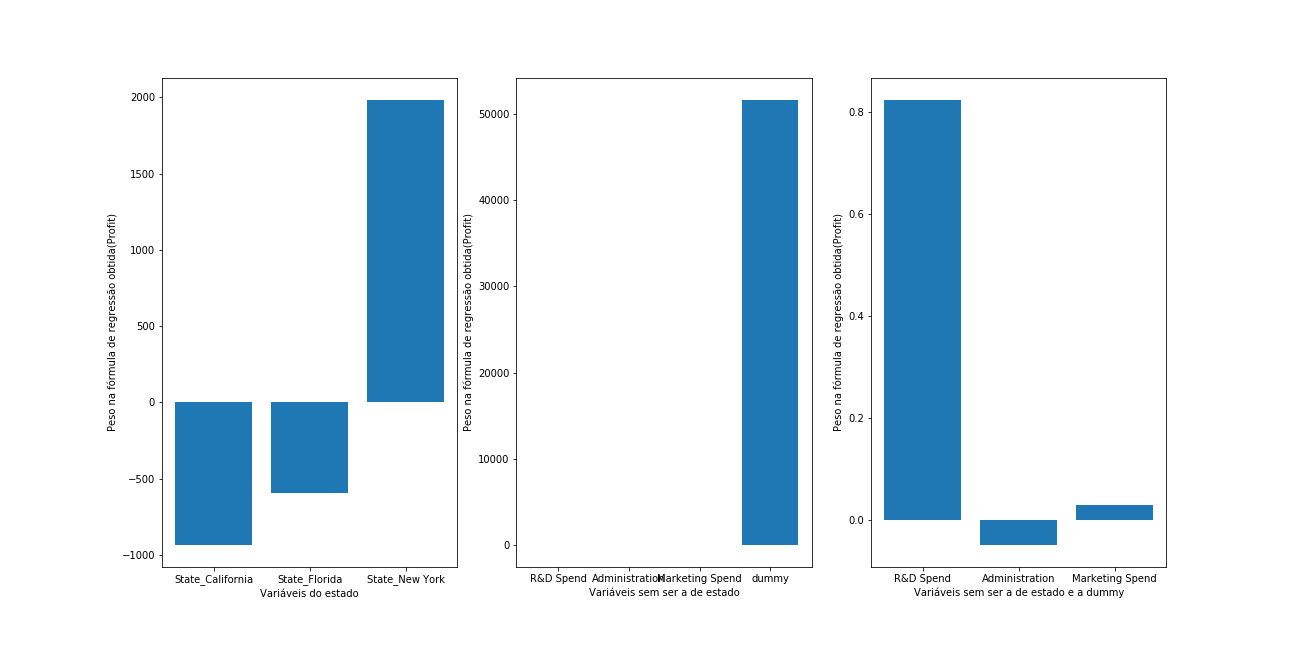
\includegraphics[width=.9\linewidth]{./cities_parameters.png}
\caption{\label{fig:parameters}
Parâmetros.}
\end{figure}


A figura \ref{fig:abs_rel_error} mostra o erro relativo e absoluto para os dados do teste. Como pode-se ver o erro relativo foi bem baixo mostrando que os valores foram bem proximos dos valores reais.

Já o erro absoluto é grande pois ele não é normalizado e isso torna difícil a análise porém pela coluna de valores reais e preditos é possivel ver que o erro foi baixo.

\begin{figure}[htbp]
\centering
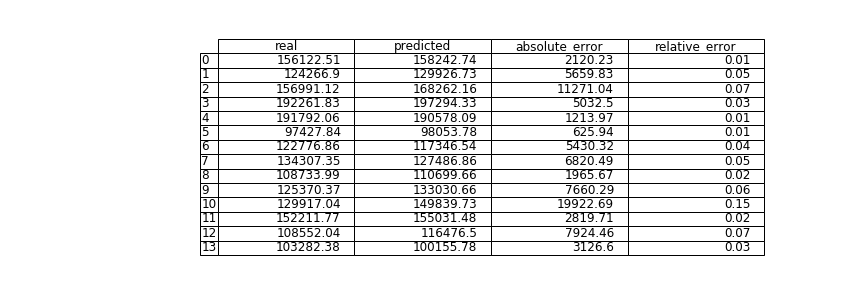
\includegraphics[width=.9\linewidth]{./abs_rel_error.png}
\caption{\label{fig:abs_rel_error}
Erros na predição dos dados no teste.}
\end{figure}

A figura \ref{fig:abs_rel_error_des} mostra os erros obtidos com medidas estatísticas, a média do erro relativo é 0.04 o que é bem baixo juntamente com o desvio padrão que também é 0.04, ou seja, o modelo criado se mostrou bem preciso.

\begin{figure}[htbp]
\centering
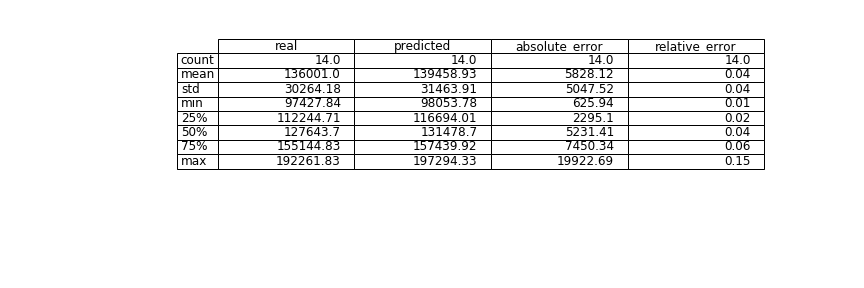
\includegraphics[width=.9\linewidth]{./abs_rel_error_des.png}
\caption{\label{fig:abs_rel_error_des}
Erros na predição dos dados no teste com medidas estatísticas.}
\end{figure}


Na figura \ref{fig:error} os erros são mostrados, tanto com a predição no teste e no treino. Por ela pode-se ver que o erro realmente foi baixo e a função de predição está descrevendo bem os dados.
Essa comprovação também foi feita pelo \(R^2\), isso pode ser visto na tabela \ref{tab:r2} que mostra um \(R^2\) proximo de 1, que significa que o modelo descreve bem os dados tanto no teste como no treino.

\begin{figure}[htbp]
\centering
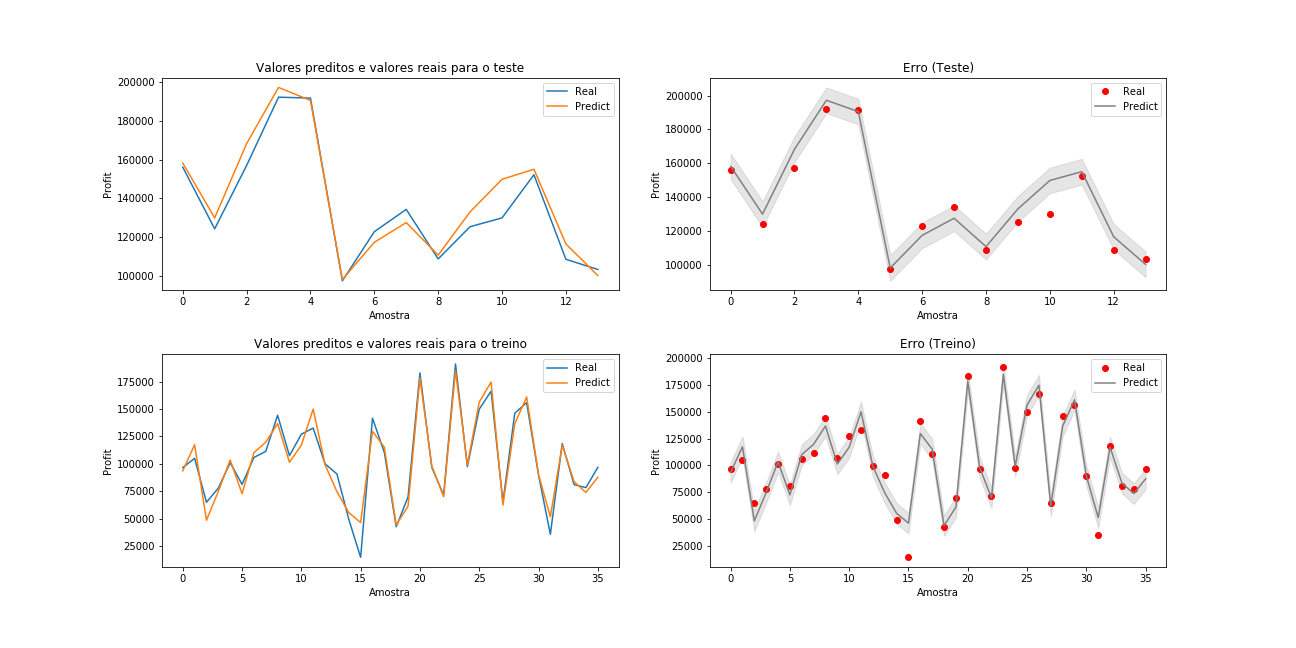
\includegraphics[width=.9\linewidth]{./error.png}
\caption{\label{fig:error}
Erros.}
\end{figure}

\begin{table}[htbp]
\centering
\begin{tabular}{lrr}
 & \(R^2\) & Adjusted \(R^2\)\\
Test & 0.93 & 0.85\\
Train & 0.94 & 0.92\\
\end{tabular}
\caption{\label{tab:r2}
\(R^2\) obtidos aplicando no treino e teste.}

\end{table}

Outros métodos de se calcular o erro foram abordados também e todos deram resultados positivos de que os erros foram baixos. (tabela \ref{tab:metrics})

\begin{table}[htbp]
\centering
\begin{tabular}{lr}
MSE & 57624666.284417234\\
RMSE & 7591.091244637838\\
RRMSE & 0.06956706362289085\\
MAE & 5828.124952610224\\
MAPE & 0.04422778830100514\\
RMSLE & 0.05537110299114828\\
\end{tabular}
\caption{\label{tab:metrics}
Diversas métricas de erro.}

\end{table}

\section{Conclusão}
\label{sec:orgf432795}

Foi possível observar que a regressão linear múltipla pode dizer muito sobre variáveis que influenciam em outras e para o problema a regressão se mostrou capaz de descrever os dados bem e com baixo erro, ou seja, o problema pode ser resolvido com regressão.

Para trabalhos futuros seria interessante comparar com outros métodos de aprendizado de maquina como por exemplo gradiente descendente e redes neurais para ver se os erros podem ser diminuídos com modelos mais complexos.
\end{document}
